\documentclass[11pt]{article}
\usepackage[margin=1in]{geometry}
% \usepackage[preprint]{neurips_2024}
\usepackage{graphicx}
\usepackage{amsmath}
\usepackage{amssymb}
\usepackage{hyperref}
\usepackage{cite}
\usepackage{titlesec}
\usepackage{float}
\usepackage{adjustbox} 
\usepackage{listings}
\usepackage{xcolor}
\usepackage{multicol}
\setcounter{secnumdepth}{4}

\title{PlantPal - helping you be a better \textit{pal} to your plants
}
\author{
    \begin{tabular}[t]{l}
        SNEHA SARKAR \\
        \texttt{A0304787U} \\
        \texttt{e1373875@u.nus.edu} \\
    \end{tabular}
    \and
    \begin{tabular}[t]{l}
        MANAV KAMLESH CHOUHAN \\
        \texttt{STUDENT\_ID} \\
        \texttt{EMAIL@u.nus.edu} \\
    \end{tabular}
    \and
    \begin{tabular}[t]{l}
        SHEN AO \\
        \texttt{STUDENT\_ID} \\
        \texttt{e1351197@u.nus.edu} \\
    \end{tabular}
    \and
    \begin{tabular}[t]{l}
        TEO XUAN WEI \\
        \texttt{STUDENT\_ID} \\
        \texttt{EMAIL@u.nus.edu} \\
    \end{tabular}
    \and
    \begin{tabular}[t]{l}
        BHUSHAN GANESH MOHOL \\
        \texttt{STUDENT\_ID} \\
        \texttt{EMAIL@u.nus.edu}
    \end{tabular}
}

\begin{document}

\maketitle

\section{Theme}
Singapore is well known for its City in a Garden vision, where greenery is integrated into urban living. With the nation’s focus on sustainability, food security, and community well-being, there is growing interest in urban farming, ornamental plant ownership, and smart agricultural solutions. Plant Pal fits into this landscape by offering an accessible digital tool for plant disease detection and care recommendations, supporting both national goals and individual needs.

\begin{enumerate}
    \item Urban Farming \& Community Gardens: Singapore has actively promoted urban farming and community gardening through NParks’ \textit{Community in Bloom} programme. Residents often cultivate herbs, orchids, and vegetables in HDB void decks, balconies, and rooftop gardens. Plant Pal can support these efforts by enabling gardeners to quickly diagnose plant diseases, ensuring healthier crops in limited urban spaces.

    \item Smart Nation \& Sustainability Goals: Aligned with the \textit{30 by 30} vision to produce 30\% of Singapore’s nutritional needs locally by 2030, local farms and nurseries face ongoing pest and disease challenges. Plant Pal offers a low-cost, scalable way to detect plant diseases early and recommend interventions, helping reduce crop losses and contributing to national food security.

    \item Relevance for Hobbyists \& Collectors: Beyond urban farming, plant ownership is a widespread hobby in Singapore. Ornamental plants such as orchids, succulents, and rare tropical foliage (e.g., monstera, philodendrons) are highly prized, with some rare orchids valued at hundreds of dollars. Plant Pal helps hobbyists protect these valuable plants by identifying early signs of disease, safeguarding both their collections and investments.
\end{enumerate}


\section{Business Model}

Plant Pal will operate on a freemium model tailored to different user groups, ensuring accessibility for hobbyists while generating sustainable revenue from farms and enterprises.

\begin{enumerate}
    \item Hobbyists \& Home Gardeners (B2C):
    \begin{itemize}
        \item Free Tier:
        \begin{itemize}
            \item Upload plant images for basic disease detection.
            \item 
            Receive general care tips and treatment suggestions.
        \end{itemize}
        \item Premium Tier (Subscription / Pay-per-use):
        \begin{itemize}
            \item Detailed diagnostic reports (disease probability, severity).
            \item Personalized plant care recommendations.
            \item Plant health tracking over time.
            \item Estimated: SGD 3–5/month or SGD 1 per premium scan.
        \end{itemize}
    \end{itemize}
    \item Community Gardens \& Small Farms (B2B Lite)
    \begin{itemize}
        \item Affordable subscription plan for groups or small farms.
        \item Features:
        \begin{itemize}
            \item Bulk scanning (multiple images per day).
            \item Data dashboard to monitor crop health trends.
            \item Seasonal advice for pest/disease prevention.
            \item Estimated: SGD 30–50/month.
        \end{itemize}
    \end{itemize}
    \item Commercial Farms \& Nurseries (B2B Enterprise)
    \begin{itemize}
        \item Tailored enterprise solution with:
        \begin{itemize}
            \item API access for integration into farm management systems.
            \item Advanced analytics on crop disease trends.
            \item Multi-user access and priority support.
            \item Pricing via custom contracts.
        \end{itemize}
    \end{itemize}
    \item Add-on Revenue Streams:
    \begin{itemize}
        \item Plant Care Marketplace: Partner with nurseries, garden shops, and agri-tech suppliers to suggest remedies (fertilizers, pesticides, soil care products) within the app. Earn referral fees or commission on sales.
        \item Data Insights: Aggregated, anonymized plant health data could support urban farming research or government food security initiatives.
    \end{itemize}
\end{enumerate}

\section{Cloud service}

Plant Pal will be deployed as a cloud-native service on AWS to ensure scalability, reliability, and accessibility for both individual users and enterprise partners. The system integrates a FastAPI backend with cloud storage, machine learning (ML) inference, and a React-based frontend.

\begin{enumerate}
    \item Core Functionality
    \begin{itemize}
        \item Plant Disease Detection API (FastAPI)
        \begin{itemize}
            \item Users upload plant images through the web interface.
            \item Images are sent to the FastAPI backend (containerized and deployed on AWS ECS or EKS).
            \item Backend triggers ML inference (plant species classification + disease detection).
            \item Output: prediction with confidence scores.
        \end{itemize}

        \item Recommendation Engine (FastAPI)
        \begin{itemize}
            \item Backend retrieves care instructions based on detected disease/species.
            \item  Advice includes watering schedules, pruning, and treatment suggestions.
        \end{itemize}

        \item User Engagement Features
        \begin{itemize}
            \item Health tracking dashboards.
            \item Notifications/reminders (via email or mobile push).
            \item Gamification (badges, streaks, milestones).
        \end{itemize}
\end{itemize}

\item Benefits of Cloud Deployment:
\begin{itemize}
    \item Scalability: ECS can auto-scale FastAPI containers during peak demand.
    \item Security: IAM roles + S3 bucket policies restrict access.
    \item Reliability: CloudFront ensures low-latency global delivery.
    \item Cost-Efficiency: Pay-per-use compute/storage; lightweight architecture for hobbyist use cases.
\end{itemize}

\end{enumerate}

\section{Preliminary design}

\begin{itemize}
    \item Frontend: React (hosted on S3 + CloudFront).
    \item  Backend: FastAPI container deployed on AWS ECS Fargate (serverless containers).
    \item Storage:
    \begin{itemize}
        \item User-uploaded images → Amazon S3.
        \item User Metadata, recommendations → Amazon DynamoDB or (SQL based RDMBS hosted on EC2).
    \end{itemize}
    \item ML Inference Layer: Hugging Face pretrained model packaged within FastAPI (for simplicity), or hosted separately on SageMaker.
    \item Authentication: AWS Cognito to manage user accounts (hobbyists, farms, admins).
    \item CI/CD: 
    \begin{itemize}
        \item GitHub Actions → deploy frontend build to S3.
        \item Dockerized FastAPI backend → pushed to ECR and deployed to ECS.
    \end{itemize}
\begin{figure}[H]
    \centering
    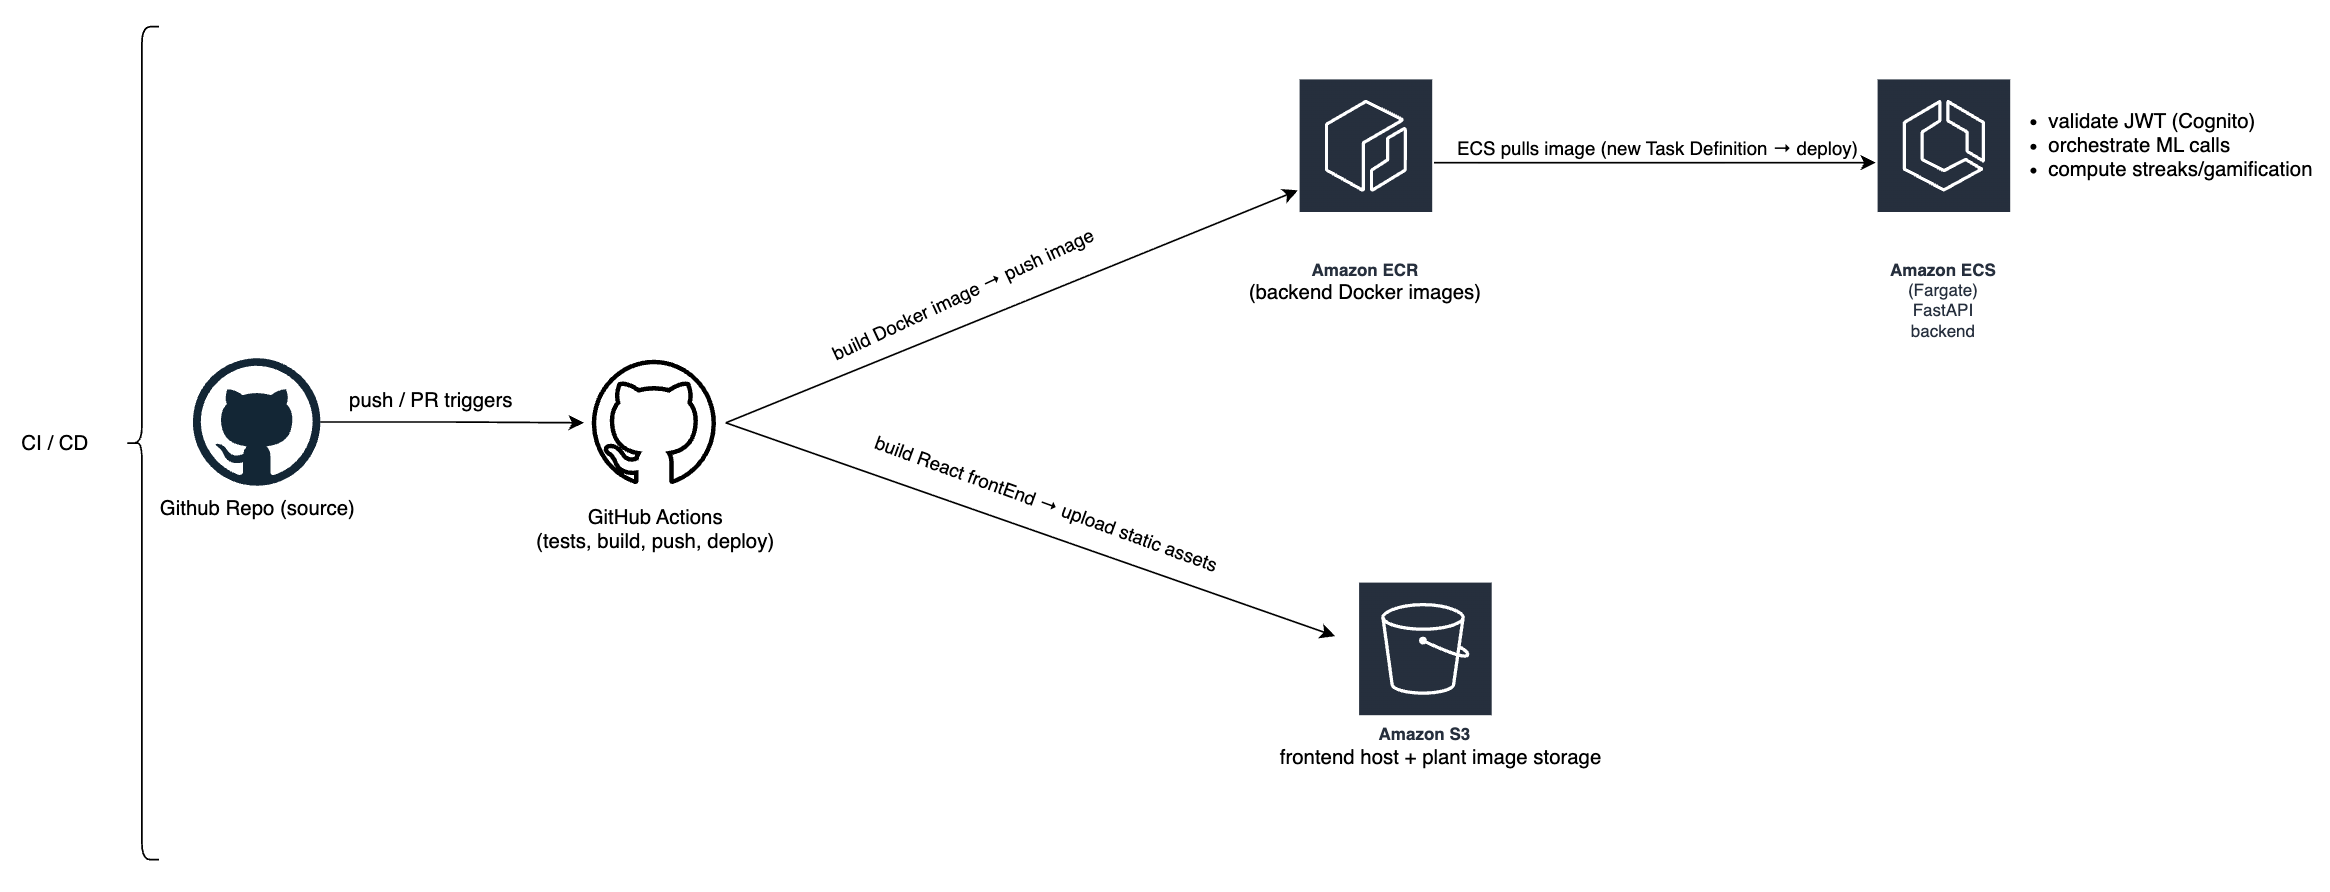
\includegraphics[width=1\linewidth]{ci_cd_pipeling.png}
    \label{fig:CI/CD Pipeline}
\end{figure}
\begin{figure}[H]
    \centering
    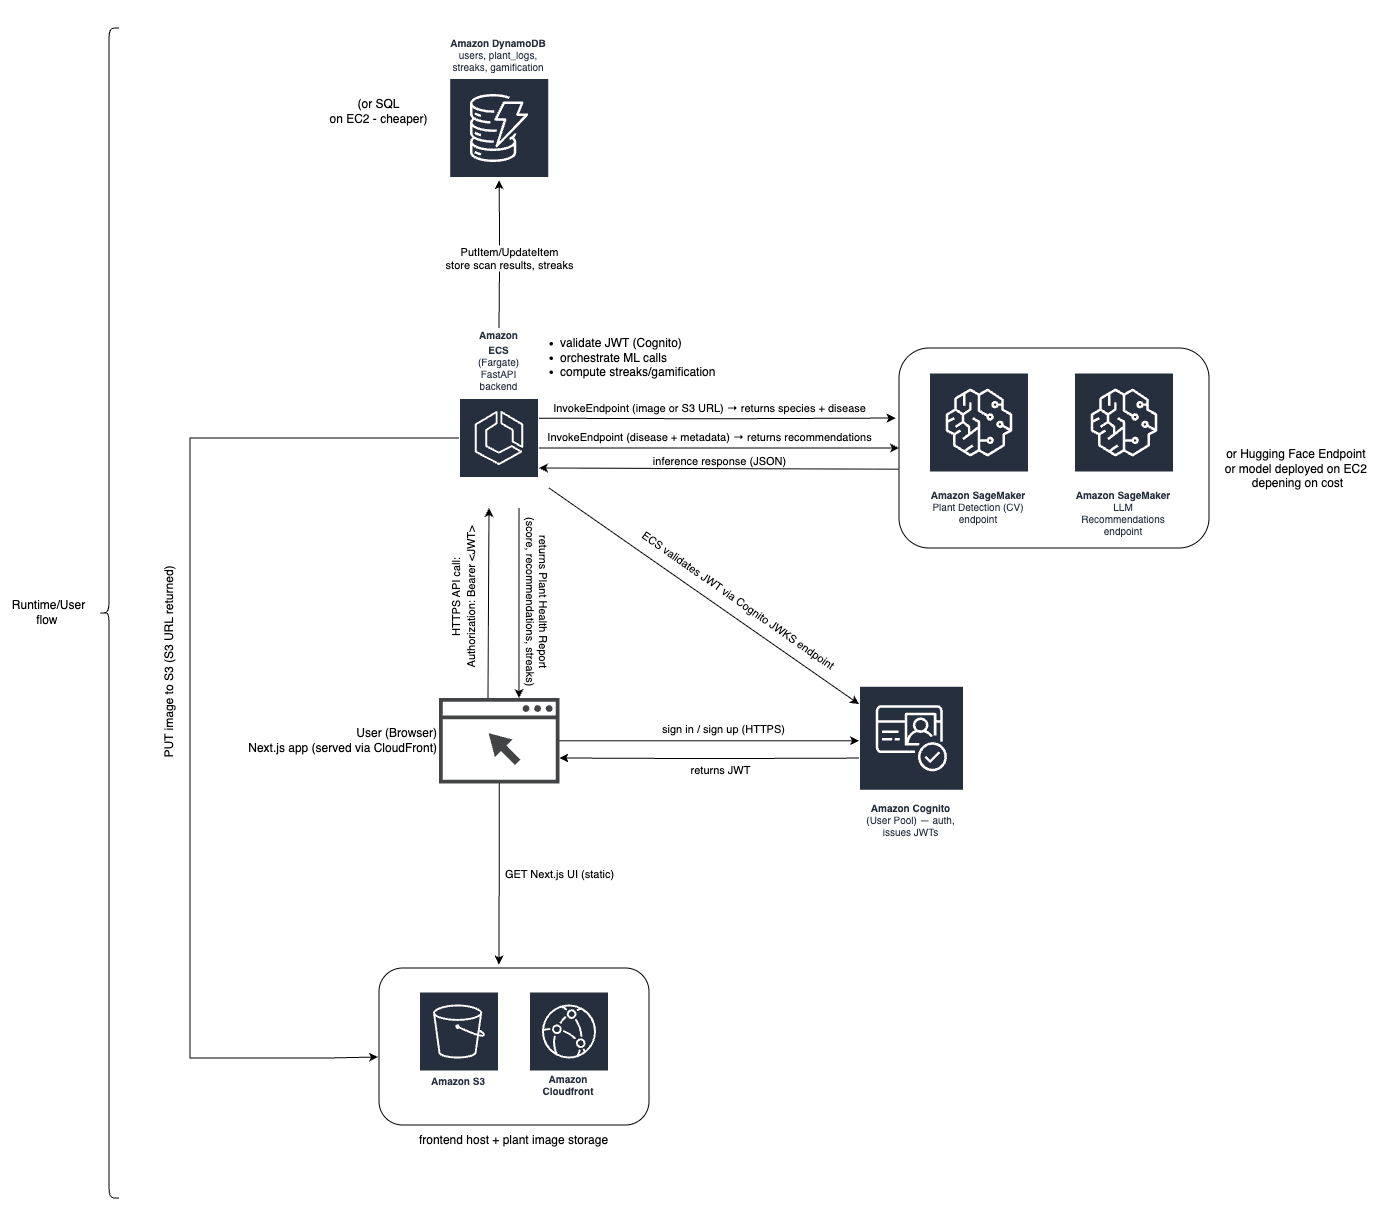
\includegraphics[width=1\linewidth]{user_flow.png}
    \label{fig:System Design}
\end{figure}
\end{itemize}

\section{Implementation plan}
\subsection*{Phase 1: Setup \& Planning}
\begin{itemize}
    \item Finalize requirements (features: plant detection, reports, streaks, authentication).
    \item Design architecture.
    \item Set up AWS accounts, GitHub repo, CI/CD skeleton.
\end{itemize}

\subsection*{Phase 2: Frontend Basics}
\begin{itemize}
    \item Build React frontend (upload photo, login/signup, dashboard, streaks).
    \item Integrate Cognito authentication $\rightarrow$ login/signup flow.
    \item Mock backend responses.
\end{itemize}

\subsection*{Phase 3: Backend Core (Weeks 3--4)}
\begin{itemize}
    \item Set up FastAPI backend in ECS (Fargate).
    \item Implement image upload $\rightarrow$ S3.
    \item Implement streaks/logging $\rightarrow$ DynamoDB / RDMBS.
    \item Connect Cognito JWT validation.
\end{itemize}

\subsection*{Phase 4: ML Integration (Weeks 5--6)}
\begin{itemize}
    \item Deploy Plant Detection model on SageMaker / HuggingFace / EC2.
    \item Deploy LLM recommendation model on SageMaker HuggingFace / EC2.
    \item Connect FastAPI $\rightarrow$ inference endpoints.
\end{itemize}

\subsection*{Phase 5: CI/CD \& Deployment (Week 7)}
\begin{itemize}
    \item CI/CD with GitHub Actions:
    \begin{itemize}
        \item Frontend $\rightarrow$ build \& deploy to S3.
        \item Backend $\rightarrow$ build Docker image $\rightarrow$ push to ECR $\rightarrow$ deploy to ECS.
    \end{itemize}
    \item Optionally monitoring via CloudWatch.
\end{itemize}

\subsection*{Phase 6: Testing \& Polishing (Week 8)}
\begin{itemize}
    \item Test full flow end-to-end: user login $\rightarrow$ upload photo $\rightarrow$ ML inference $\rightarrow$ report + streaks.
    \item Fix bugs, polish UI, add gamification touches (leaderboard, streak badges).
\end{itemize}


\end{document}



 